\ylDisplay{Plokid} % Ülesande nimi
{Tundmatu autor} % Autor
{lõppvoor} % Voor
{2012} % Aasta
{P 7} % Ülesande nr.
{3} % Raskustase
{
% Teema: Mehaanika

\ifStatement
Liikuva ploki abil on võimalik saavutada jõus kahekordne võit (vt joonis). Joonistage sellised plokkide süsteemid, mille kasutamisel koorma tõstmiseks on jõu võit: a) $5$-kordne; b) $2,5$-kordne.
\begin{center}
	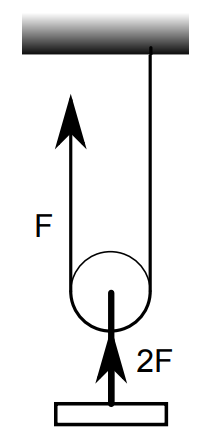
\includegraphics[width=0.5\linewidth]{2012-v3p-07-yl.PNG}
\end{center}
\fi

\ifHint
Mitmekordse jõu võidu saamiseks on vaja sellised plokisüsteemid panna üksteise suhtes järjestikku. Poolekordset võitu saab jällegi, kui ülesandes toodud süsteemi rakendada vastupidiselt.
\fi

\ifSolution
\begin{center}
	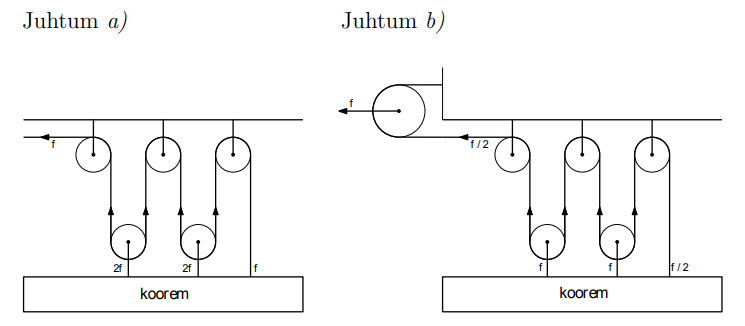
\includegraphics[width=0.5\linewidth]{2012-v3p-07-lah.PNG}
\end{center}
\fi
}